\chapter*{Notaci\'{o}} \addcontentsline{toc}{chapter}{Notaci\'{o}}

Es presenta a continuaci\'{o} la notaci\'{o} seguida en aquest llibre.

Cal fer notar que les variables vectorials i matricials s'escriuen
en lletra negreta inclinada,  mentre que les variables escalars
s'escriuen en lletra normal inclinada.

\begin{list}{}
{\setlength{\labelwidth}{15mm} \setlength{\leftmargin}{20mm}
\setlength{\labelsep}{5mm}}
    \item[$\ju$] La unitat imagin\`{a}ria, definida com:
    $\ju\equiv\sqrt{-1}$\index{j}
    \item[$V$] Una variable real.
    \item[$\cmplx{V}$] Una variable complexa.
    \item[$\cmplx{V}^*$] Conjugat d'una variable complexa.
    Es compleixen les relacions:\\[1ex]
     $(\cmplx{V}_1 \pm \cmplx{V}_2 \pm \cdots  \pm \cmplx{V}_n)^* = \cmplx{V}_1^* \pm
    \cmplx{V}_2^*\pm\cdots\pm\cmplx{V}_n^*$\\[1ex]
    $(\cmplx{V}_1 \cmplx{V}_2 \cdots \cmplx{V}_n)^* = \cmplx{V}_1^*  \cmplx{V}_2^*
    \cdots \cmplx{V}_n^*$\\[1ex]
    $(\cmplx{V}_1 / \cmplx{V}_2)^* = \cmplx{V}_1^* / \cmplx{V}_2^*$
    \item[$|\cmplx{V}|$] M\`{o}dul d'una variable complexa.
    Es compleixen les relacions:\\[1ex]
      $\cmplx{V}\cmplx{V}^* = |\cmplx{V}|^2$\\[1ex]
      $1/ \cmplx{V} = \cmplx{V}^* / \,|\cmplx{V}|^2$\\[1ex]
      $|\cmplx{V}_1 \cmplx{V}_2 \cdots \cmplx{V}_n| =
       |\cmplx{V}_1| \,|\cmplx{V}_2| \cdots |\cmplx{V}_n|$\\[1ex]
       $|\cmplx{V}_1 / \cmplx{V}_2| = |\cmplx{V}_1| \,/ \,|\cmplx{V}_2|$\\[1ex]
      $|\cmplx{V}_1+\cmplx{V}_2+\cdots+\cmplx{V}_n| \leq
      |\cmplx{V}_1| + |\cmplx{V}_2| + \cdots  +|\cmplx{V}_n|$
    \item[$\arg(\cmplx{V})$] Argument (angle) d'una variable complexa.
     Es compleixen les relacions:\\[1ex]
      $\arg(\cmplx{V}^*) = - \arg(\cmplx{V})$\\[1ex]
      $\arg(\cmplx{V}_1 \cmplx{V}_2 \cdots \cmplx{V}_n) = \arg(\cmplx{V}_1) + \arg (\cmplx{V}_2) + \cdots + \arg(\cmplx{V}_n)$\\[1ex]
      $\arg(\cmplx{V}_1 / \cmplx{V}_2) = \arg(\cmplx{V}_1) - \arg (\cmplx{V}_2)$
    \item[$\Re(\cmplx{V})$] Part real d'una variable complexa. Es compleix: $\Re(\cmplx{V}) = \dfrac{\cmplx{V} + \cmplx{V}^*}{2}$
    \item[$\Im(\cmplx{V})$] Part imagin\`{a}ria d'una variable complexa. Es compleix: $\Im(\cmplx{V}) = \dfrac{\cmplx{V} - \cmplx{V}^*}{2 \ju}$
    \item[$A+\ju B$] Expressi\'{o} cartesiana (part real i part
    imagin\`{a}ria) d'una variable complexa.
    \item[$Z_{\angle \psi}$] Expressi\'{o} polar (m\`{o}dul i argument) d'una variable
    complexa. Les relacions entre $A, B, Z$ i $\psi$\footnote{Cal tenir en compte que la funci\'{o} \textsf{arctan} disponible en moltes calculadores i llenguatges de programaci\'{o}, torna de forma  estandarditzada valors compresos entre $-\frac{\piup}{2}$ i $\frac{\piup}{2}$. En aquest cas cal sumar el valor $\piup$, quan $A$ \'{e}s negatiu, a l'angle obtingut amb la funci\'{o} \textsf{arctan} per tal d'obtenir l'angle en el quadrant correcte.} s\'{o}n:\\[1ex]
    $Z=+\sqrt{A^2+B^2}\quad\quad\psi=\arctan{\dfrac{B}{A}}\quad\quad
    A=Z\cos\psi\quad\quad B=Z\sin\psi$
    \item[$Z\,\eu^{\ju\psi}$] Expressi\'{o} d'Euler\index{Euler} d'una variable complexa, definida com:
     $Z\,\eu^{\ju\psi} \equiv Z(\cos\psi+\ju\sin\psi)$.
     Es compleixen les relacions:\\[1ex]
     $Z_1\,\eu^{\ju\psi_1} \, Z_2\,\eu^{\ju\psi_2} = Z_1 Z_2\,\eu^{\ju(\psi_1+\psi_2)}$\\[1ex]
     $(Z_1\,\eu^{\ju\psi_1}) \,/\, (Z_2\,\eu^{\ju\psi_2}) = \dfrac{Z_1}{Z_2}\,\eu^{\ju(\psi_1-\psi_2)}$
    \item[$\boldsymbol{V}$] Una matriu real o un vector real.
    \item[$\boldsymbol{V}^{-1}$] Matriu inversa d'una matriu real.
    \item[$\transp{\boldsymbol{V}}$] Matriu transposada d'una matriu real o vector
    transposat d'un vector real.
    \item[$\boldsymbol{V}(n)$] Element $n$-\`{e}sim d'un vector real.
    \item[$\boldsymbol{V}(m,n)$] Element de la fila $m$ i columna $n$ d'una matriu real.
    \item[$\mcmplx{V}$] Una matriu complexa o un vector complex.
    \item[$\mcmplx{V}^{-1}$] Matriu inversa d'una matriu complexa.
    \item[$\transp{\mcmplx{V}}$] Matriu transposada d'una matriu complexa o vector
    transposat d'un vector complex.
    \item[$\mcmplx{V}^*$] Matriu conjugada d'una matriu complexa o vector
    conjugat d'un vector complex.
    \item[$\hermit{V}$] Matriu conjugada transposada d'una matriu complexa o vector
    conjugat transposat d'un vector complex, definit com: $\hermit{V} \equiv
    \transp{(\mcmplx{V}^*)}$.
    \item[$\mcmplx{V}(n)$] Element $n$-\`{e}sim d'un vector complex.
    \item[$\mcmplx{V}(m,n)$] Element de la fila $m$ i columna $n$ d'una matriu complexa.
\end{list}

Pel que fa als sentits assignats a les fletxes que representen les
tensions i els corrents en els diversos circuits el\`{e}ctrics que
apareixen en aquest llibre, s'utilitza la convenci\'{o} seg\"{u}ent:

\begin{list}{}
{\setlength{\labelwidth}{15mm} \setlength{\leftmargin}{20mm}
\setlength{\labelsep}{5mm}}
    \item[$\begin{CD} @>U>> \end{CD}$] Tensi\'{o} cont\'{\i}nua; la fletxa indica el sentit
    de la caiguda de tensi\'{o}, \'{e}s a dir, va del nus positiu al nus negatiu.
    \item[$\begin{CD} @>I>> \end{CD}$] Corrent
    continu; la fletxa indica el sentit  assignat com a positiu al corrent.
    \item[$\begin{CD} @>\cmplx{U}>> \end{CD}$] Tensi\'{o} alterna; la fletxa indica el
    sentit assignat com a positiu a la caiguda de tensi\'{o}, quan el nus d'origen de la fletxa
    t\'{e} un potencial  m\'{e}s positiu que el nus de destinaci\'{o}.
    \item[$\begin{CD} @>\cmplx{I}>> \end{CD}$] Corrent altern; la fletxa
    indica el sentit  assignat com a positiu al corrent.
\end{list}

\pagebreak

En aquest llibre les variable complexes s'utilitzen per representar fasors. Un fasor $V_{\angle \alpha}$ representa la funci\'{o} sinuso\"{\i}dal variable en el temps: $v(t)=\sqrt{2}\, V \cos(\omega t + \alpha)$. El par\`{a}metres implicats s\'{o}n:
\begin{list}{}
{\setlength{\labelwidth}{15mm} \setlength{\leftmargin}{20mm}
\setlength{\labelsep}{5mm}}
    \item[$v(t)$] Funci\'{o} sinuso\"{\i}dal; representa normalment una tensi\'{o} o un corrent.
    \item[$t$] Temps.
    \item[$f$] Freq\"{u}\`{e}ncia de la funci\'{o} sinuso\"{\i}dal.
    \item[$T$] Per\'{\i}ode de la funci\'{o} sinuso\"{\i}dal.
    \item[$\omega$] Velocitat angular de la funci\'{o} sinuso\"{\i}dal. Es compleix: $\omega = 2 \piup f = 2 \piup\,/T$.
    \item[$V$] Valor efica\c{c} de la funci\'{o} sinuso\"{\i}dal (vegeu la secci\'{o} \vref{sec:val_mitja_ef}); el valor de pic de la funci\'{o} sinuso\"{\i}dal \'{e}s:  $\pm\sqrt{2}\, V$.
    \item[$\alpha$] Angle inicial de la funci\'{o} sinuso\"{\i}dal. Es compleix:  $\alpha=\omega t_0$ (vegeu el gr\`{a}fic a continuaci\'{o}); $\alpha$ \'{e}s positiu quan es mesura des de l'origen cap a l'esquerra, fins a trobar el primer valor m\`{a}xim de la funci\'{o} sinuso\"{\i}dal, i \'{e}s negatiu quan es mesura des de l'origen cap a la dreta, fins a trobar tamb\'{e} el primer valor m\`{a}xim de la funci\'{o} sinuso\"{\i}dal.
    \item[] 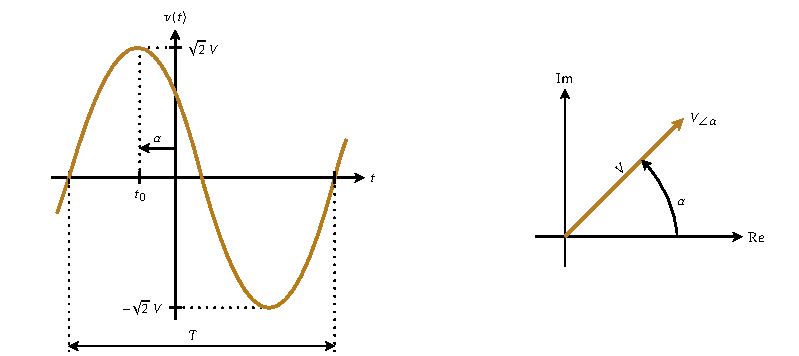
\includegraphics{Imatges/Not-Fasor.pdf}
\end{list}
\index{fasor}

Els s\'{\i}mbols que representes els diferents conjunts de nombres s\'{o}n:

\begin{list}{}
{\setlength{\labelwidth}{15mm} \setlength{\leftmargin}{20mm}
\setlength{\labelsep}{5mm}}
    \item[$\mathbb{Z\phantom{{}^+}}$] Nombres enters: $\ldots,-2,-1,0,1,2,\ldots$
    \item[$\mathbb{N}$, $\mathbb{Z}^+$] Nombres enters positius
    (naturals): $1,2,3,4,\ldots$
    \item[$\mathbb{Z}^*\,$] Nombres enters no negatius: $0,1,2,3,4,\ldots$
    \item[$\mathbb{Z}^-$] Nombres enters negatius: $-1,-2,-3,-4,\ldots$
    \item[$\mathbb{Q\phantom{{}^+}}$] Nombres racionals.
    \item[$\mathbb{R\phantom{{}^+}}$] Nombres reals.
    \item[$\mathbb{R}^+$] Nombres reals positius.
    \item[$\mathbb{R}^-$] Nombres reals negatius.
    \item[$\mathbb{C\phantom{{}^+}}$] Nombres complexos.
\end{list}
\index{n@$\mathbb{N}$} \index{z@$\mathbb{Z}$}
\index{z@$\mathbb{Z^+}$} \index{z@$\mathbb{Z^-}$}
\index{z@$\mathbb{Z^*}$} \index{q@$\mathbb{Q}$}
\index{r@$\mathbb{R}$} \index{r@$\mathbb{R^+}$}
\index{r@$\mathbb{R^-}$} \index{c@$\mathbb{C}$}
